\chapter{High-dimensional limit of two-layer neural networks} \label{chap:context}
\chaptermark{High-dimensional limit of two-layer NN}

In this Chapter, we introduce the core object of the entire work: \emph{soft committee machines},
a special case of two-layer neural networks.
We also define the dynamics that we are going to study and rephrase the training in terms
of more convenient variables. Using some well-known results in the literature, we derive the 
\emph{ordinary differential equations} describing the process, which will be the starting point 
for all further analysis in the work.

To conclude, we present some results obtained, as an example of 
outcomes using this setting.

\section{The setting}
The setting we are going to present was first introduced by Saad \& Solla \cite{saad1995line}
back in 1995,
and it is often named after them.
In recent years, this framework has been used as starting point in many different papers
\cite{aubin2018committee, goldt2019dynamics,veiga2022phase}.

We are going to do the same in this work; we present the exact same setting of the seminal paper \cite{saad1995line}, while the differences
will appear in the next chapters. We will also briefly expose some more recent results \cite{goldt2019dynamics},
that put some mathematical rigor in the derivation of the differential equations.

\subsection{Online Gradient Descent on Soft Committee Machines}
Let's consider a two-layer neural network, with the input layer of dimension \(d\),
a hidden layer of arbitrary dimension and the output layer constituted by just 1 node.
In addition, the weight between the hidden layer and the output layer are all fixed 
to the same constant; the activation function \(\act(\cdot)\) is applied only in hidden layer nodes.
The assumptions of using one single neuron with fixed weights can be relaxed without any additional effect appearing in the model.
Training the second layer would complicate the notation, without adding value to the analysis we want to conduct;
for reference to work that does not fix the second layer see Goldt et al.\cite{goldt2019dynamics}.
We, therefore, limit our investigation to the simplest model that captures all the effects of interest to us.
\begin{figure}
  \centering
  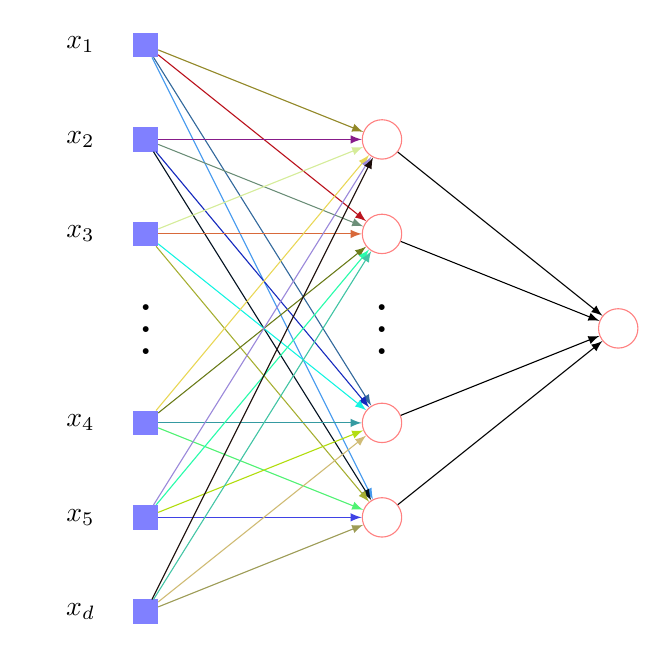
\begin{tikzpicture}[x=1.5cm, y=1.2cm, >=latex]
    \tikzset{
  inputnode/.style={
    rectangle,
    draw,
    minimum size=.3cm
  },
  every neuron/.style={
    circle,
    draw,
    minimum size=.5cm
  },
  neuron missing/.style={
    draw=none, 
    fill=none, %<- added
    scale=2,
    text height=0.333cm,
    execute at begin node=\color{black}$\vdots$
  }
}

\pgfmathparse{rnd}
\xdefinecolor{MyColor}{rgb}{\pgfmathresult, 1.0, 1.0}

\foreach \m [count=\y] in {1,2,3,missing,4,5,6} %<- removed "/\l" here 
  \node [fill=black,inputnode/.try, neuron \m/.try,blue!50] (input-\m) at (0,2.5-\y) {};
% added "fill=green" in the line above

\foreach \m [count=\y] in {1,2,missing,3,4}
  \node [every neuron/.try, neuron \m/.try,red!50] (hidden-\m) at (2,1.5-\y) {};

\foreach \m [count=\y] in {1}
  \node [every neuron/.try, neuron \m/.try,red!50] (output-\m) at (4,-.5-\y) {};

\foreach \l [count=\i] in {1,2,3,4,5,d}
  \path (input-\i) -- ++(-1,0)
   node [midway] {$x_\l$};

% \foreach \l [count=\i] in {1,n}
%   \draw [->] (output-\i) -- ++(1,0)
%    node [above, midway] {$a_\l$};

\foreach \i in {1,...,6}
  \foreach \j in {1,...,4} {
    \edef\R{\pdfuniformdeviate 255}
    \edef\G{\pdfuniformdeviate 255}
    \edef\B{\pdfuniformdeviate 255}
    \xdefinecolor{MyColor}{RGB}{\R,\G,\B}
    \draw [->,MyColor] (input-\i) -- (hidden-\j);
  }


\foreach \i in {1,...,4}
  \foreach \j in {1}
    \draw [->] (hidden-\i) -- (output-\j);

% \foreach \l [count=\x from 0] in {Eingangs-, Ausgangs-}
%   \node [align=center, above] at (\x*4,2) {\l \\ Neuronen};
  \end{tikzpicture}
  \caption{ schematic view of a soft committee machine.
            Different colors represent different weights; the output perceptron has uniform weights.}
\end{figure}
This is known in Statistical Physics literature as the \emph{soft
committee machine}. The name comes from a pictorial representation where every hidden neuron can be seen 
as a member of a committee that independently takes a ``decision'' based on the input;
the final answer of the machine is then obtained by combining the output of the committee
members in a single value. Moreover, the attribute \emph{soft} comes from the fact
that all the members (a.k.a hidden neurons) have the same weight.

We aim to study the training of such a model under some strong assumptions that will
allow us to derive some analytical properties of the entire process.
In particular, we assume the existence of a \emph{teacher} capable to give the output
value at any given input. The teacher is a soft committee machine too, and it is defined 
by a function \(f\colon \Real^d\to\Real\), where \(d\) is the dimension
of the input; the dimension of the teacher's hidden layer is \(k\),
while the matrix of weights \(\W^* \in \Real^{k\times d}\).
The function takes the form
\[
  f{(\vec{x})} = \frac{1}{k}\sum_{r=1}^{k} \act{\left(\frac{\vec{w}^*_r \cdot \vec{x}}{\sqrt{d}}\right)}
  \quad\text{where}\quad \vec{w}^*_r \coloneqq [\W^*]_r \in \Real^d. 
\]
We emphasize that the choice of weights for the second layer was made so that
the output is the average of the values of the hidden neurons. This choice allows
us to compare the output of networks with different hidden layer sizes.
We maintain this convention for all soft committee machines considered in this work.

The machine that are we going to train using the \emph{teacher} output is called \emph{student}.
This particular choice is called \emph{teacher-student setting} and is often used
as a toy model to study the properties of some more complicated problems.
We emphasize that the student knows nothing about the architecture of the teacher.
The teacher is just a convenient generative model for the data and the student observes only the pairs of labels and points,
not the architecture of the teacher.
This might appear as an unfaithful representation of a real situation since it is hardly credible 
that the samples are generated from a model analogous to the one we want to study.
Still, we use this assumption because, as we show later, it allows us to write convenient
variables to monitor and study the learning.
Moreover, in this way we also have the guarantee that the distribution of data is learnable by the student;
if not, we may miss some of the learning steps we want to study.

The student function of course has a similar structure to the teacher.
The only differences are the size of the hidden layer, which is \(p\),
and the weights, which will be  \(\W \in \Real^{d\times p}\). In addition, the weights are not constant
throughout the learning process; we use the apex \(\nu\) to indicate the weights after \(\nu\) steps of learning.
The function of the student is
\[
  \hat{f}^\nu{(\vec{x})} = \frac{1}{p}\sum_{j=1}^{p} \act{\left(\frac{\vec{w}^\nu_j \cdot \vec{x}}{\sqrt{d}}\right)}
  \quad\text{where}\quad \vec{w}^\nu_j \coloneqq [\W^\nu]_j \in \Real^d. 
\]

We make one more assumption in our study: the distribution of the input samples is
normal and independent on each component.
Independence is crucial in order to obtain equations that can be treated analytically,
while the precise distribution is not. 
If desired, we could study non-Gaussian distributions as done by Refinetti~et~al.~\cite{refinetti2022dynamics},
but this would only lead to a complication of calculations, without having a truly more general model.
Moreover, even independence does not make the input used lose generality,
as there are techniques to make the inputs independent, such as principal component analysis.
Using formulas, the samples \(\left(\vec{x}^\nu, y^\nu\right) \in \Real^{d\times1}\) 
used to train the student are chosen as
\[
  \vec{x}^\nu \sim \gauss{(0,\I_d)} \quad\text{ and }\quad 
  y^\nu = f{(\vec{x}^\nu) + \sqrt{\Delta}\xi^\nu}\quad\text{with } \xi^\nu \sim \gauss{(0,1)}.
\]
The value of \(\Delta\ge0\) regulates the noise we are adding to the teacher signal.
The presence of noise is intended to emulate the fact that in a real situation the 
data is not perfect, but it is subject to disturbances of different kinds.
In general, the presence of noise makes the task harder.

The most known and used methods for the neural networks are the many different 
versions of the \emph{gradient descent}. Usually, in supervised learning,
there is a finite dataset where every sample is used in many different learning
steps (possibly all). This reflects the fact that the amount of information accessible
to train the network is finite; it happens more often than you might think, however,
the amount of data available is larger than the amount that can be computed, so one single sample is just used once.
We are going to use what is called the \emph{online gradient descent}
(also known as \emph{one-pass gradient descent}); at each learning step one new sample
is generated from the assumed distribution, used only once and then discarded.
This emulates real situations of data overabundance, but more importantly, it allows us
to write deterministic equations that describe the process since we need the independence
of different learning steps.

Given all the consideration we did and fixing the \emph{learning rate} at \(\gamma>0\),
the update rule of the student weights is
\begin{equation} \label{eq:update_rule_weights}
  \w^{\nu+1}_j = \w^{\nu}_j - \gamma \nabla_{\w_j}\left(\loss\left(y^\nu,\hat{f}^{\nu-1}{\left(\vec{x}^\nu\right)}\right)\right),
\end{equation}
where \(\loss\) is the loss function.
We know that, in order to get the better learning possible, the learning rate should
be chosen so that it decreases as the training progresses, but this does not fundamentally change the stages of learning,
which is ultimately what we want to study; we, therefore, make the choice to hold the learning rate constant for simplicity.
For an analysis that takes into account the possibility of the learning rate varying, see Veiga~et~al.~\cite{veiga2022phase}.

The Equation \eqref{eq:update_rule_weights} is called \emph{update rule for the weights},
and it essentially define a discrete stochastic process. %todo: maybe expand this

The last thing we have to specify for the gradient descent is the loss function \(\loss\).
The choice we did is the \emph{mean squared error}
\[
  \loss{\left(y^\nu,\hat{f}^{\nu-1}{\left(\vec{x}^\nu\right)}\right)} = \frac{1}{2}\left(y^\nu-\hat{f}^{\nu-1}{\left(\vec{x}^\nu\right)}\right)^2.
\]
The final goal of the training is to minimize the \emph{theoretical risk}
(or \emph{population error}), defined as
\begin{equation} \label{eq:theoretical_risk_definition}
  \risk^{\nu} = \E_{\vec{x}\sim\gauss{(0,\I_d)}}{
  \left[\loss{\left(f{\left(\vec{x}\right)},\hat{f}^\nu{\left(\vec{x}\right)}\right)}\right]}=
  \frac{1}{2}\E_{\vec{x}\sim\gauss{(0,\I_d)}}{\left[\left(f{\left(\vec{x}\right)}-\hat{f}^{\nu}{\left(\vec{x}\right)}\right)^2\right]}.
\end{equation}
We have access to this quantity just because we are working in the teacher-student setting.
In real world, one can only monitor the learning using the \emph{empirical risk}, an estimation
of the theoretical one given by the known samples.
This is of course a feature of our artificial setup,
which simply allows us to have complete control of the training.
We emphasize the fact that theoretical risk is not used for the learning step
(it is never the argument of the gradient), but only for monitoring.

We should mention that for the online gradient descent in particular (and not for other types of GD),
the limit \(\gamma\to0\) converges to the gradient flow dynamics on theoretical risk \cite{chizat2019lazy}.
This is a very interesting theoretical fact, which would deserve a separate discussion,
but since we would stray too far from our discussion (we are not studying this limit,
for us the learning rate is a finite quantity), we defer the interested readers to the references.




\subsection{Local Fields and Macroscopic variables}
Looking at the Equation \eqref{eq:theoretical_risk_definition} it's easy to realize
that the risk depends only on the value of the weights, both of the student and of the
teacher. In particular, the weights fully describe the status of a committee machine.
Along the lines of what is done in statistical physics, we would like to define \emph{macroscopic variables}
that do not contain all the information about how the neural network is constructed,
but still be descriptive of its state. In particular, we are interested in expressing
the risk only in function of these variables.
In other words, we are not interested in having control over the state of the weights,
which in thermodynamic language will be the microscopic variables,
but we only need to monitor enough statistics to calculate population risk.

We start the derivation of the macroscopic variables by defining the \emph{local fields}
\[
  \vec{\lf}^{\nu} = \frac{\W^{\nu}\vec{x}}{\sqrt{{d}}} \quad\text{and}\quad
  \vec{\lf}^{*\nu} = \frac{\W^{*}\vec{x}}{\sqrt{{d}}},
\]
where the apices \({\nu+1}\) on \(\vec{x}\) are omitted since they don't matter,
as shown hereafter. These are just the values of the hidden layers, before applying 
the activation function. They are interesting because the whole setting can be rephrased
in terms of the local fields, forgetting the existence of \(\vec{x}^\nu\).
The functions \(f\), \(\hat{f}\) and \(\risk\) depend only on the local fields and not explicitly
on \(\vec{x}^\nu\), therefore it's sufficient to sample and track local fields in order to monitor the learning.
As we already said many times, this is possible just because we are in the artificial
teacher-student setting, but it does not make the analysis less deep.

The \(\vec{\lf}\)s are linear combinations of normal random variables, so they are
normal too. We can then extract some sufficient statics to characterize them.\\
Let's start from the mean, which is particularly straightforward since the \(\vec{x}\)s
are all 0-mean
\[
  \E_{{\vec{x}\sim\gauss{(0,\I_d)}}}{\left[\lf_j^\nu\right]} = \E_{{\vec{x}\sim\gauss{(0,\I_d)}}}{\left[\lf_r^{*\nu}\right]} = 0
  \qquad \forall j\in[p], r\in[k].
\]
It follows that the only quantity needed to characterize the local fields is 
the covariance matrix. 
Let's start with the student-student covariance
\[\begin{split}
  \E_{{\vec{x}\sim\gauss{(0,\I_d)}}}{\left[\lf_j^\nu\lf_l^\nu\right]} &= 
  \E_{{\vec{x}\sim\gauss{(0,\I_d)}}}{\left[\frac1d w_{ja}x_a w_{lb}x_b\right]} =
  \frac1dw_{ja}w_{lb}\E_{{\vec{x}\sim\gauss{(0,\I_d)}}}{\left[x_ax_b\right]}\\ &= 
  \frac1dw_{ja}w_{lb} \delta_{ab} = \frac1dw_{ja}w_{la} = \frac{\left[\W^\nu\W^{\nu\top}\right]_{jl}}{d},\\
\end{split}\]
The other terms are completely analogous
\[
  \E_{{\vec{x}\sim\gauss{(0,\I_d)}}}{\left[\lf_j^\nu\lf_r^{*}\right]} = \frac{\left[\W^\nu\W^{*\top}\right]_{jr}}{d}
  \quad\text{and}\quad
  \E_{{\vec{x}\sim\gauss{(0,\I_d)}}}{\left[\lf_r^*\lf_t^{*}\right]} = \frac{\left[\W^*\W^{*\top}\right]_{rt}}{d}.
\]

The covariance matrices of local fields are a perfect candidate to be
the macroscopic variables we are looking for. Therefore, we give an explicit 
definition of what are known as the \emph{order parameters}
\begin{equation} \label{eq:order_parameters_definiton}
  \Q^\nu \coloneqq \frac{\W^\nu \W^{\nu\top}}{d}, \qquad
  \M^\nu \coloneqq \frac{\W^\nu \W^{*\top}}{d} \quad\text{and}\quad
  \P \coloneqq \frac{\W^* \W^{*\top}}{d}.
\end{equation}
Let us look more closely at these newly defined matrices. \(\Q\) is a square symmetric
matrix of dimension \(p\times p\), where each entry is the overlap between the two
weights of the student. Likewise, \(\P\) is square symmetric, but of dimension \(k\times k\);
it's the auto-overlap of the teacher. Moreover, \(\P\) does not change throughout
the process since the teacher weights are not update. Instead, \(\M\) is a \(p\times k\)
matrix, where each entry is the overlap between a neuron of the teacher and a neuron
of the student. Lastly, \(M\) has more rows than column, the student perfectly 
learns the teacher when has just one non-zero entry per column, each one on a different row.

All covariances can be assembled into a single matrix
\[
  \vec{\Omega}^\nu \coloneqq \left(\begin{array}{cc}
    \Q^\nu & \M^\nu \\
    % \hline
    \M^{\nu\top} & \P
  \end{array}\right).
\]
The matrix \(\vec{\Omega}\in\Real^{(p+k)\times(p+k)}\) is called \emph{overlap matrix} and it fully
describes the learning since it can be used as the covariance matrix for sampling the local fields.
In fact, the local fields at step \(\nu+1\) of the learning can be written as random variables with distribution
\[\vec{\lf}^{\nu+1},\vec{\lf}^{*\nu+1} \sim \gauss{(0,\vec{\Omega}^\nu)}.\]

To conclude this Subsection, we redefine the teacher and the student function
in terms of just the local fields
\[
  f{(\vec{\lf^*})} = \frac{1}{k}\sum_{r=1}^{k} \act{\left(\lf^*_r\right)}\quad\text{and}\quad
  \hat{f}{(\vec{\lf^{\nu}})} = \frac{1}{p}\sum_{j=1}^{p} \act{\left(\lf_j\right)}.
\]
These two lead also to an expression of theoretical risk in terms of overlap matrix only, 
by taking an expected value on local fields
\begin{equation}\label{eq:riskfunctionalOmega}
  \risk{(\vec{\Omega})} = \frac12\E_{\vec{\lf},\vec{\lf^* \sim \gauss{(0,\vec{\Omega})}}}
                              {\left[\left(f{(\vec{\lf}^*)} - f{(\vec{\lf})}\right)^2\right]}
  \quad\text{and}\quad\risk^\nu \equiv \risk{\left(\vec{\Omega}^\nu\right)}.
\end{equation}
We have explicitly expressed the quantity of our interest in terms of the macroscopic 
variables only; the next step is to eliminate the need for weights to describe the learning process.





\subsection{Update rule for overlap matrix} \label{subsec:updateruleforoverlap}
In the previous Subsection, we introduced the order parameters and we showed that 
they are sufficient to describe the status of the learning. We would now like
to write the evolution as a function of only the order parameters,
so we can treat them as the only dynamic quantity of the system.
The goal is therefore to have an update rule for \(\vec{\Omega}\).
First of all, we introduce the \emph{displacement}
\[
  \dsp^\nu \coloneqq f{(\vec{\lf}^*)} - \hat{f}{(\vec{\lf})} + \sqrt{\Delta} \xi^\nu,
\]
as a quantity that just lightens the notation.
Given this definition, the loss function evaluated at \((\vec{x}^\nu,y^\nu)\)
can be simply written as
\[\loss{\left(y^\nu,\hat{f}^{\nu-1}{\left(\vec{x}^\nu\right)}\right)} = \frac{\left(\dsp^\nu\right)^2}{2}.\]
Consequently, the expression of the population risk can be written with this notation As
\begin{equation}\label{eq:risk_lambda_expval}
  \risk{(\vec{\Omega})} = \frac12\E_{\vec{\lf},\vec{\lf^* \sim \gauss{(0,\vec{\Omega})}}}
                              {\left[\left(\dsp^\nu\right)^2\right]}.
\end{equation}

The second step is to explicitly compute the gradient of the loss respect to the weights
\[
  \nabla_{\w_j}\left(\frac{\left(\dsp^\nu\right)^2}{2}\right) =
    -\dsp^\nu \nabla_{\w_j}\left(\hat{f}{\left(\vec{\lf_j}\right)}\right) =
    -\dsp^\nu \frac{\act'{\left(\vec{\lf}^\nu_j\right)}}{p}\frac{\vec{x}^\nu}{\sqrt{d}} =
    -\frac{1}{p}\dsp^\nu_j \frac{\vec{x}^\nu}{\sqrt{d}},
\]
where in the last step we used another notation shorthand
\[
  \dsp^\nu_j \coloneqq \act'{(\lambda_j^\nu)} \dsp^\nu.
\]
We stress out the fact that all the \(\dsp\) and \(\dsp^\nu\) are in the end function of only
the local fields.

Indeed, it follows from Equation \eqref{eq:update_rule_weights} that the update rule
for the weights still depends on the sample \(\vec{x}^\nu\)
\[
  \w^{\nu+1}_j = \w^{\nu}_j + \frac{\gamma}{p} \dsp^\nu_j \frac{\vec{x}^\nu}{\sqrt{d}}.
\]

We can now use this to derive the update rules for the order parameters.
Let's start from \(\M\)
\begin{equation} \label{eq:update_rule_M}
  \left[\M^{\nu+1}\right]_{jr} = \frac{\w^{\nu+1}_j \w^{*\top}_r}{d}
    = \frac{\w^{\nu}_j \w^{*\top}_r}{d} + \frac{\gamma}{dp} \dsp^\nu_j \frac{\vec{x}^\nu}{\sqrt{d}}\w^{*\top}_r
    = \left[\M^{\nu}\right]_{jr} + \frac{\gamma}{dp} \dsp^\nu_j \lf_r^*,
\end{equation}
that is not explicitly dependent in \(\vec{x}\) or \(\vec{w}\). The computation
for the \(\Q\) update rule is a little bit more complex
\begin{equation}\label{eq:update_rule_Q}\begin{split}
  \left[\Q^{\nu+1}\right]_{jl} &= \frac{\w^{\nu+1}_j \w^{\nu+1\top}_l}{d}
    = \frac{\w^{\nu}_j \w^{\nu\top}_l}{d} + \frac{\gamma}{pd} \dsp^\nu_j \frac{\vec{x}^\nu}{\sqrt{d}}\w_l^\nu
      + \frac{\gamma}{pd} \dsp^\nu_l \frac{\vec{x}^\nu}{\sqrt{d}}\w_j^\nu 
      + \frac{\gamma^2}{p^2d} \dsp^\nu_j\dsp^\nu_l \frac{\left(\vec{x}^\nu\right)^2}{d}\\
    &= \left[\Q^{\nu}\right]_{jl} + \frac{\gamma}{pd}\left(\dsp^\nu_j \lf_l^\nu + \dsp^\nu_l \lf_j^\nu\right)
    + \frac{\gamma^2}{p^2d} \dsp^\nu_j\dsp^\nu_l \frac{\left(\vec{x}^\nu\right)^2}{d}.
\end{split}\end{equation}
We notice that the update rule still depends explicitly on \(\vec{x}^\nu\).
Apparently, this dependence prevents us from being able to write an update rule
that depends only on order parameters and local fields, but, as we show now, the 
high-dimensional is of help.
In fact, the factor \(\frac{\left(\vec{x}^\nu\right)^2}{d}\) goes to 1 and 
fluctuations can be neglected, in the limit of large \(d\) and fixed \(p,k,\gamma\) and \(\Delta\)\footnote{
  \(\left(\vec{x}^\nu\right)^2\) is distributed as a Chi-square with \(d\) degrees
  of freedom, so for large \(d\) we have 
  \(\frac{\left(\vec{x}^\nu\right)^2}{d} \sim \gauss{\left(1,\frac1d\right)}\).

  Although it is a passage often found in the literature,
  this statement is not obvious and especially not rigorous.
  For simplicity's sake, we report as it is.
  In the next section we will give a formal justification on how to go from update rule
  to differential equations; the theorem we present also includes this unclear step.
}. Consequently, as of now, we will no longer write this term, assuming it has been replaced by 1.

In conclusion, learning can be described as a \emph{discrete stochastic process}
on the overlap matrix
\[\left\{\vec{\Omega}^\nu \in \Real^{(p+k)\times(p+k)}|\nu\in\Natural\right\},\]
and the risk is just a function of \(\vec{\Omega}\), as shown in Equation~\eqref{eq:riskfunctionalOmega}.
We succeeded in transforming our setting built to study the learning of a neural network,
in a simpler stochastic process of some macroscopic variables, that do not fully characterize
the network, but still give enough information for further analysis.





\subsection{High-dimensional limit}
In this Subsection we proceed in expressing the most important result of Saad\&Solla\cite{saad1995line}:
the derivation of \emph{ordinary differential equations} whose solution can be used
to approximate the stochastic process of the order parameters. 

We first present a derivation \emph{à la physicist}, that gives a great intuition of what is going on,
but it lacks mathematical rigor. After that, we briefly present some recent results that
formalize the idea.
We stick to the Saad-Solla regime, where there is no dependence in \(d\) of \(p\) and \(\gamma\).

The thing to point out is how to pass from a discrete process to a time-continuous equation.
In other words, we need a mapping from the step number \(\nu\) to a time \(t\) such that
the discretization becomes finer and finer the closer we approach the limit of higher dimension.
The update rules for the macroscopic variables can be manipulated to obtain
\begin{subequations}\label{eq:order_param_discrete_derivative}\begin{align}
  \frac{\left[\M^{\nu+1}\right]_{jr} - \left[\M^{\nu}\right]_{jr}}{\frac1d} &= \frac{\gamma}{p} \dsp^\nu_j \lf_r^*\\
  \frac{\left[\Q^{\nu+1}\right]_{jl} - \left[\Q^{\nu}\right]_{jl}}{\frac1d} &=
    \frac{\gamma}{p}\left(\dsp^\nu_j \lf_l^\nu + \dsp^\nu_l \lf_j^\nu\right) + \frac{\gamma^2}{p^2} \dsp^\nu_j\dsp^\nu_l.
\end{align}\end{subequations}
If we force the left-hand side to become a derivative in the limit, the natural choice at this point is the time scaling is
\[t=\frac{\nu}{d} \quad\text{and}\quad \delta{t} =\frac1d.\]
We now have to take the limit for \(d\to\infty\) (or analogously \(\delta t \to 0\))
As already said, the LHSs of the equations above turn into a continuous time derivative.
The tricky part is the right-hand side: the increase of dimension can be seen as 
an increase of i.i.d. random variables on which average on. This picture is true
because the \(\vec{x}\) only appears through local fields, where is first scalar-multiplied
by a weights vector, and then divided by a scaling \(\sqrt{d}\). 
% \todo{Questa parte é spiegata con i piedi!}
We can then invoke a heuristic version of the central limit theorem,
and state that the random variables appearing at the RHS converge in the limit
to their expected value. All these claims turn out to be true, so we can finally write
\begin{subequations}\label{eq:genericODE}\begin{align}
  \label{eq:genericODEforM}
  \dod{\left[\M{\left(t\right)}\right]_{jr}}{t} &=\E_{\vec{\lf},\vec{\lf^* \sim \gauss{(0,\vec{\Omega}{(t)})}}}{\left[\frac{\gamma}{p} \dsp_j \lf_r^*\right]} \eqqcolon \Psi_{jr}{\left(\vec{\Omega}\right)}\\
  \label{eq:genericODEforQ}
  \dod{\left[\Q{\left(t\right)}\right]_{jl}}{t} &=\E_{\vec{\lf},\vec{\lf^* \sim \gauss{(0,\vec{\Omega}{(t)})}}}{\left[\frac{\gamma}{p}\left(\dsp_j \lf_l + \dsp_l \lf_j\right) + \frac{\gamma^2}{p^2} \dsp_j\dsp_l\right]} \eqqcolon \Phi_{jl}{\left(\vec{\Omega}\right)},
\end{align}\end{subequations}
where we have also defined the two matrix function \(\vec{\Psi}\colon\Real^{(p+k)\times(p+k)} \to\Real^{p\times k}\) and 
\(\vec{\Phi}\colon\Real^{(p+k)\times(p+k)} \to\Real^{p\times p}\).
They are well-defined because the local fields are 0-mean gaussian, so any statics
can only depend on their covariance matrices.

In short, the discrete stochastic process has turned into a continuous deterministic evolution.
For some choices of the activation function, the expectations can be computed analytically and
the so derived system of ordinary differential equations can be studied in order
to understand the learning process.

\subsubsection{Formal derivation}
In this part, we briefly present an important result by Goldt et al.\cite{goldt2019dynamics}
that achieves to give some mathematical rigor to the derivation of the differential
equations. It also provides a bound on the maximum expected error between the process
and the equations' solution. We are not going to report the full proof, but just 
present the main theorem, explaining clearly all the hypotheses and regimes in which
it is applicable.

The original Theorem is valid for any kind of committee machine, but we only present
an adaptation to the \emph{soft} case, to be consistent with the notation
we introduced in the previous sections.
\begin{theorem}\label{thm:process_to_ode_goldt}
  Let's suppose that
  \begin{enumerate}
    \item The function \(\sigma\) is bounded and its derivatives up to the second order exist and are bounded, too;
    \item The initial macroscopic state \(\vec{\Omega^0}\) is deterministic and bounded by a constant;
    \item The constants \(\Delta, p, k\) and \(\gamma\) are all finite.
  \end{enumerate}
  Let \(T>0\), then the overlap matrix satisfies 
  \begin{equation}
    \max_{0\le\nu\le Td} \E\left[
      \left\|\vec{\Omega}^\nu - \tilde{\vec{\Omega}}\left(\frac{\nu}{d}\right)\right\|
    \right]
    \le
    \frac{C{(T)}}{\sqrt{d}},
  \end{equation}
  where \(\tilde{\vec{\Omega}}\) it's the unique solution of the Equations \eqref{eq:genericODE},
  with the initial condition \(\tilde{\vec{\Omega}}{(0)} = \vec{\Omega}^0\). 
\end{theorem}
The important part is that the constant \(C{(T)}\) does not depend on \(T\), thus 
the theorem proves the convergence of the ODEs solution to the stochastic process.
The proof can be found in the original paper\cite{goldt2019dynamics};
it is strongly based on some techniques introduced by Wang in some previous works
\cite{wang2017scaling,wang2019solvable}.

Thanks to the Theorem, we have formal proof that the well-known Equations~\eqref{eq:genericODE}
can be used to analyze the learning of a committee machine. From this point,
we assume the \emph{differential equations} to be descriptive of our system,
and we will use them to derive different kinds of results.

%todo: forse bisognerebbe dire altro, ma per ora mi va bene cosí.



\section{Example: Phase Diagram of Soft Committee Machine}
In this Section, we are going to present the results obtained by Veiga et al.\cite{veiga2022phase},
as an example of the application of all the tools introduced in the previous section.
This paper was the starting point for the work we present in this thesis;
discussions with the authors helped to arrive at the results of this thesis.
Therefore, we believe that reporting the results can likewise help the understanding of the next chapters,
as well as show the potential of the tools we have just exposed.

The setting we presented in the last Section assumed that \(p\) and \(\gamma\) were constant when the limit \(d\to\infty\) was calculated.
The purpose of the paper is to extend this analysis to the case where both network width and learning rate depend polynomially on \(d\).
We arrive at drawing a phase diagram for the final state of learning as a function of the scaling exponents of \(p\) and \(d\).

Suppose that \(p\) and \(\gamma\) vary as a function of \(d\) as
\[p=p_0 d^\kappa\quad\text{and}\quad\gamma=\gamma_0d^{-\delta}.\]
All the derivation made in the previous section, up to before the limit procedure,
also applies when using the substitutions above. We can then rewrite the Equations~\eqref{eq:order_param_discrete_derivative}
in this context
\begin{subequations}\label{eq:order_param_discrete_derivative}\begin{align}
  \left[\M^{\nu+1}\right]_{jr} - \left[\M^{\nu}\right]_{jr} &= \frac{1}{d^{1+\kappa+\delta}}\frac{\gamma_0}{p_0} \dsp^\nu_j \lf_r^*,\\
  \left[\Q^{\nu+1}\right]_{jl} - \left[\Q^{\nu}\right]_{jl} &=
  \frac{1}{d^{1+\kappa+\delta}}\frac{\gamma_0}{p_0}\left(\dsp^\nu_j \lf_l^\nu + \dsp^\nu_l \lf_j^\nu\right) + \frac{1}{d^{1+2(\kappa+\delta)}}\frac{\gamma_0^2}{p_0^2} \dsp^\nu_j\dsp^\nu_l.
\end{align}\end{subequations}
The time differential that is used to make the limit is no longer simply \(1/d\),
but depends explicitly on \(\kappa\) and \(\delta\)
\[
  \delta t = \max\left(\frac{1}{d^{1+\kappa+\delta}}, \frac{1}{d^{1+2(\kappa+\delta)}}\right).
\]
What happens when we go to the limit \(d\to+\infty\) is that, depending on the value of \(\kappa+\delta\),
some terms in the equations are suppressed, thus leading to very different differential equations and consequently different results in learning.
We can distinguish the following 4 regimes:
\begin{itemize}
  \item \emph{Plateau} \(\kappa = -\delta\): the equations obtained are exactly the same as the previous Section.
        The learning process converges to a plateau related to the noise value.
        In any case, the result has been extended, since we previously knew it was valid only for \(\kappa=\delta=0\);
  \item \emph{Perfect Learning} \(\kappa > -\delta\): the risk at the end of the learning process goes to zero, even in the presence of noise.
  \item \emph{Bad learning} \(-\frac12<\kappa+\delta<0\): the linear terms in \(\gamma_0/p_0\) in the equations are suppressed;
        the noise dominates the learning process and it's not guaranteed that the final value of the risk is smaller than the starting value.
  \item \emph{No ODEs} \(\kappa+\delta<-\frac12\): the stochastic process can't be described with ODEs, since some terms does not concentrate.
\end{itemize}
\begin{figure}
  \centering
  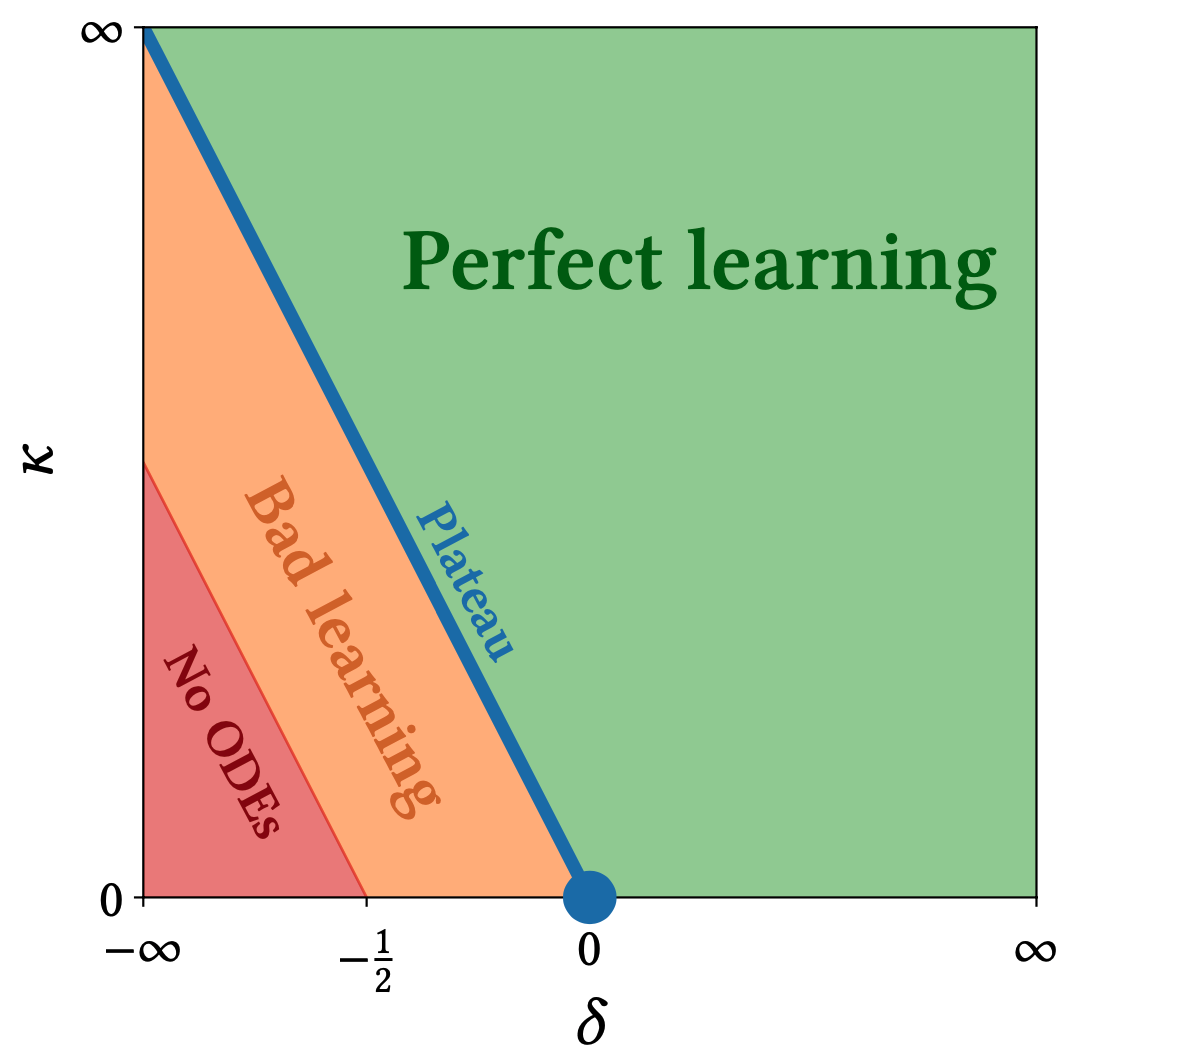
\includegraphics[width=0.7\textwidth]{figures/veiga_phase_diagram.png}
  \caption{
    schematic phase diagram showing the different regimes.
    Source~\cite{veiga2022phase}.
  }
  \label{fig:veiga_phase_diagram}
\end{figure}
\begin{figure}
  \centering
  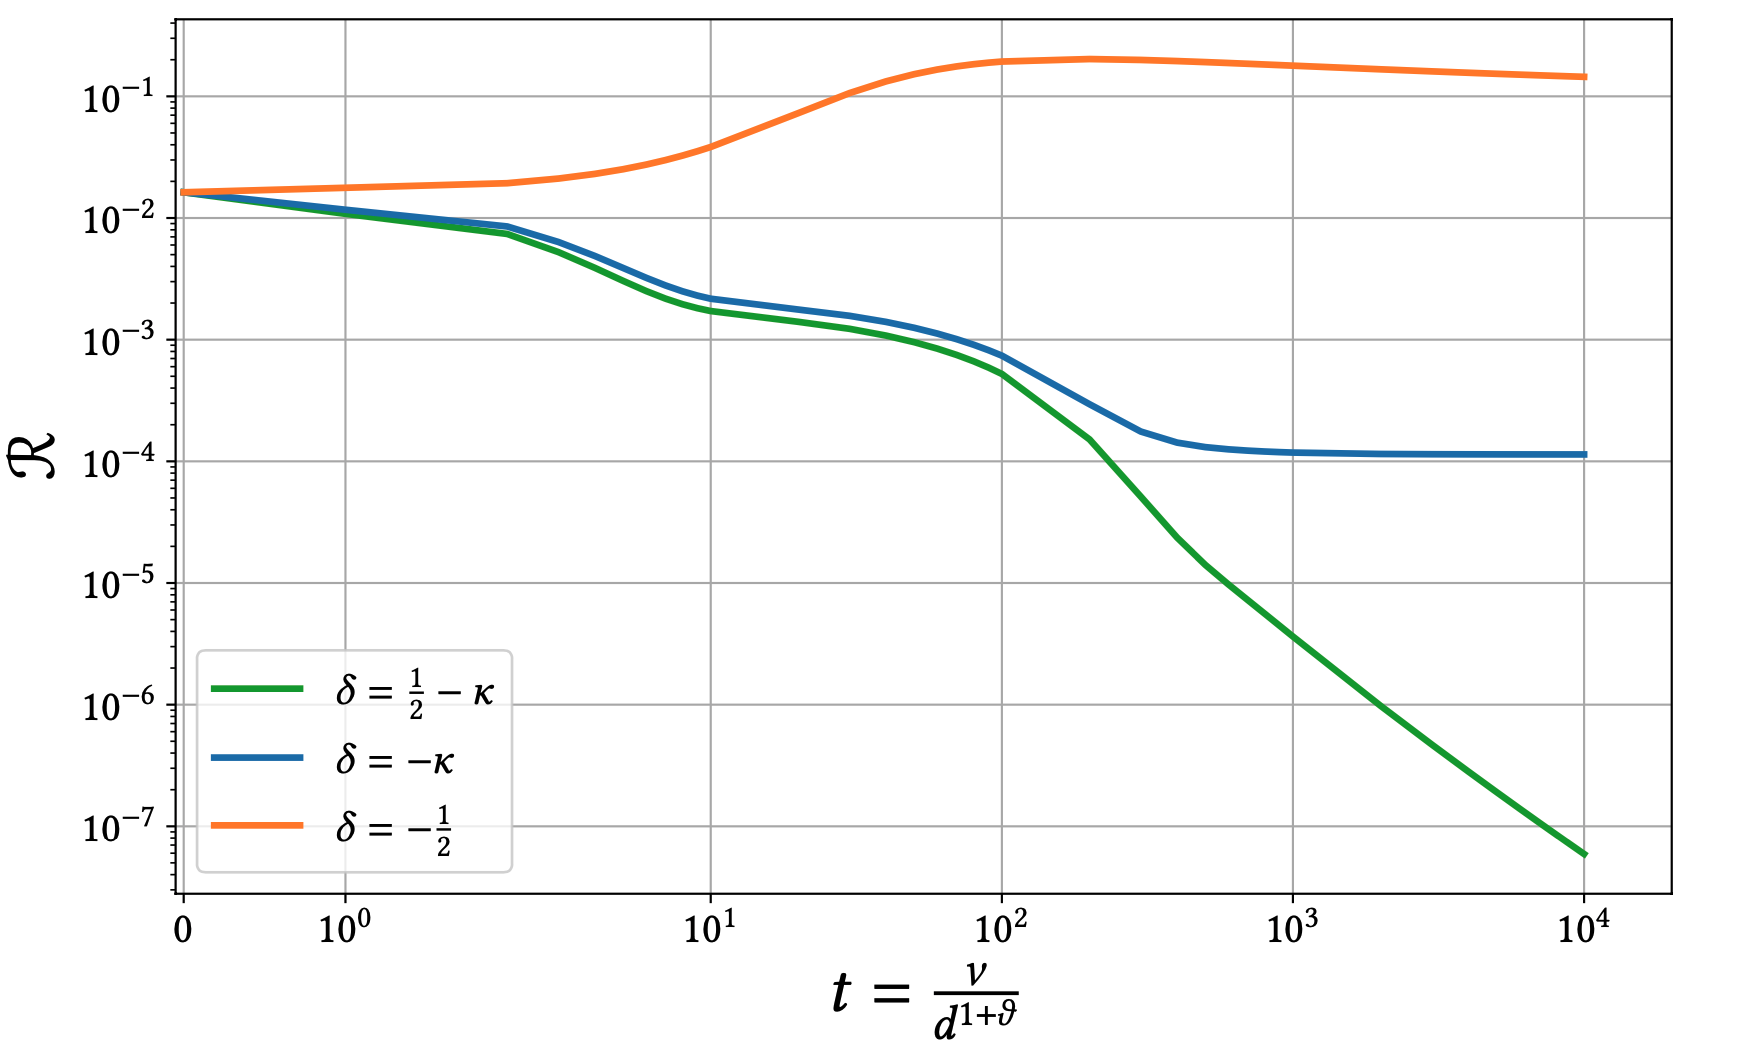
\includegraphics[width=0.9\textwidth]{figures/veiga_traj_examples.png}
  \caption{
    example of trajectories in different regimes. Yellow: bad learning; blue: plateau; green: perfect learning.
    Source~\cite{veiga2022phase}.
  }
  \label{fig:veiga_traj_examples}
\end{figure}
Figure~\ref{fig:veiga_phase_diagram} is a schematic representation that summarizes the 4 different regimes.
Figure~\ref{fig:veiga_traj_examples} shows simulated trajectories in different regimes, supporting what we presented.
The interesting thing is that if the learning rate decreases you always have perfect learning; however, this is not a necessary condition: if the network is large enough even if the learning rate diverges you can still have perfect learning.

We also note that the case we are going to study (\(\kappa=\delta=0\)) is in a very special regime ``on the edge of learning''.
We, however, will not be interested in the end state, but we would like to study the dynamics leading up to it.
In particular, we will focus on estimating the transition times of the various stages of learning.
